\begin{figure}[tbp]
\centering
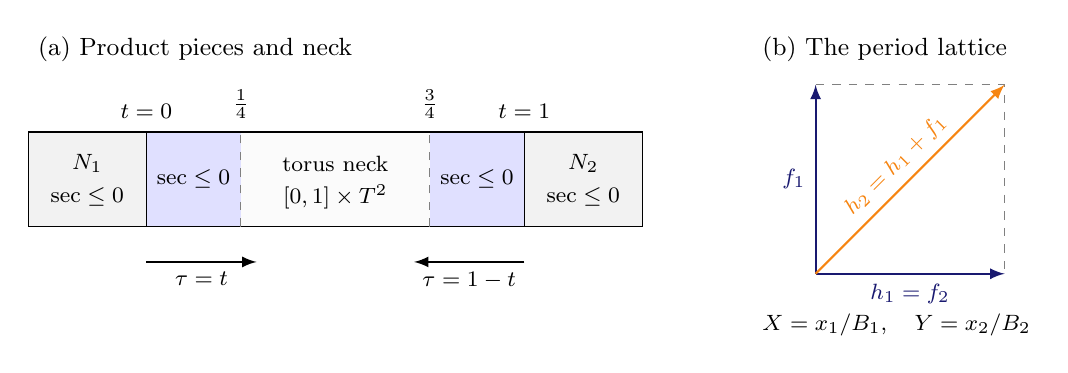
\begin{tikzpicture}[x=1cm,y=1cm,>=latex,font=\footnotesize]
  \node[anchor=west,font=\small] at (0,3.15)
    {(a) Product pieces and neck};
  \fill[gray!10] (0,0.9) rectangle (1.5,2.1);
  \fill[gray!10] (6.3,0.9) rectangle (7.8,2.1);
  \fill[Blue!12] (1.5,0.9) rectangle (2.7,2.1);
  \fill[Blue!12] (5.1,0.9) rectangle (6.3,2.1);
  \fill[gray!3] (2.7,0.9) rectangle (5.1,2.1);
  \draw (0,0.9) rectangle (7.8,2.1);
  \draw (1.5,0.9) -- (1.5,2.1);
  \draw (6.3,0.9) -- (6.3,2.1);
  \draw[dashed,gray] (2.7,0.9) -- (2.7,2.1);
  \draw[dashed,gray] (5.1,0.9) -- (5.1,2.1);
  \node at (0.75,1.7) {$N_1$};
  \node at (7.05,1.7) {$N_2$};
  \node at (0.75,1.28) {$\sec\le0$};
  \node at (7.05,1.28) {$\sec\le0$};
  \node at (2.1,1.5) {$\sec\le0$};
  \node at (5.7,1.5) {$\sec\le0$};
  \node at (3.9,1.7) {torus neck};
  \node at (3.9,1.28) {$[0,1]\times T^2$};
  \node[above] at (1.5,2.15) {$t=0$};
  \node[above] at (2.7,2.15) {$\frac14$};
  \node[above] at (5.1,2.15) {$\frac34$};
  \node[above] at (6.3,2.15) {$t=1$};
  \draw[->,thick] (1.5,0.45) -- (2.9,0.45)
    node[midway,below] {$\tau=t$};
  \draw[->,thick] (6.3,0.45) -- (4.9,0.45)
    node[midway,below] {$\tau=1-t$};

  \node[anchor=west,font=\small] at (9.2,3.15)
    {(b) The period lattice};
  \draw[dashed,gray] (10,2.7) -- (12.4,2.7) -- (12.4,0.3);
  \draw[->,thick,MidnightBlue] (10,0.3) -- (12.4,0.3)
    node[midway,below] {$h_1=f_2$};
  \draw[->,thick,MidnightBlue] (10,0.3) -- (10,2.7)
    node[midway,left] {$f_1$};
  \draw[->,thick,BurntOrange] (10,0.3) -- (12.4,2.7)
    node[midway,above,sloped] {$h_2=h_1+f_1$};
  \node[anchor=west] at (9.2,-0.35)
    {$X=x_1/B_1,\quad Y=x_2/B_2$};
\end{tikzpicture}
\caption{The construction in schematic coordinates.  Each product piece
$N_i$ includes its convex collar; the two end portions of the neck also have
nonpositive sectional curvature.  The arrows indicate the inward
coordinate at each end.  The lattice cell is drawn in normalized
coordinates $(X,Y)$: since $B_1=\epsilon B_2$, its diagonal represents
$h_2=B_2(e_2+\epsilon e_1)=h_1+f_1$ even when the coordinate shear
$\epsilon$ is small.  Physical lengths are not to scale, and drawn angles
are not angles of the Riemannian metric.}
\label{fig:neck-gluing}
\end{figure}
